% !TeX TS-program = txs:///duck
\documentclass{standalone}
\usepackage{tikzducks}

\begin{document}
	
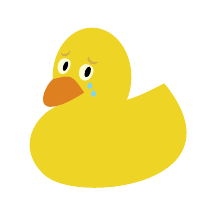
\begin{tikzpicture}
	\duck[grumpy,eye=yellow!70!brown]
	\fill[white!85!yellow] (0.9121,1.5426) .. controls (0.9357,1.6075) and (0.9015,1.6397) .. (0.8552,1.6566) .. controls (0.8088,1.6735) and (0.7652,1.6477) .. (0.7442,1.6038) .. controls (0.7205,1.5388) and (0.7390,1.4725) .. (0.7853,1.4557) .. controls (0.8317,1.4388) and (0.8885,1.4777) .. (0.9121,1.5426) -- cycle (0.6199,1.6197) .. controls (0.6415,1.6790) and (0.6260,1.7156) .. (0.5852,1.7304) .. controls (0.5443,1.7453) and (0.4937,1.7328) .. (0.4721,1.6735) .. controls (0.4505,1.6141) and (0.4661,1.5540) .. (0.5069,1.5391) .. controls (0.5477,1.5243) and (0.5983,1.5603) .. (0.6199,1.6197) -- cycle;
	\fill[black, rotate=-20] (0.26,1.7575) ellipse (0.0357 and 0.0714);
	\fill[black, rotate=-20] (-0.03,1.73) ellipse (0.0286 and 0.0643);
	\fill[yellow!30!brown] (0.9778,1.6871) .. controls (0.9011,1.6753) and (0.8740,1.7030) .. (0.8531,1.7606) .. controls (0.8034,1.6833) and (0.9421,1.6177) .. (0.9778,1.6871) -- cycle (0.6229,1.8394) .. controls (0.5901,1.7822) and (0.5420,1.7734) .. (0.4966,1.8048) .. controls (0.5213,1.7300) and (0.6310,1.7565) .. (0.6229,1.8394) -- cycle;		
	\fill[cyan!50!white] (0.9026,1.3929) .. controls (0.9135,1.3706) and (0.8889,1.3471) .. (0.8719,1.3471) .. controls (0.8549,1.3471) and (0.8303,1.3706) .. (0.8412,1.3929) .. controls (0.8519,1.4148) and (0.8549,1.4150) .. (0.8719,1.4388) .. controls (0.8827,1.4099) and (0.8904,1.4182) .. (0.9026,1.3929) -- cycle (0.9499,1.2931) .. controls (0.9608,1.2707) and (0.9362,1.2472) .. (0.9192,1.2472) .. controls (0.9022,1.2472) and (0.8776,1.2708) .. (0.8885,1.2931) .. controls (0.8992,1.3150) and (0.9022,1.3151) .. (0.9192,1.3389) .. controls (0.9300,1.3100) and (0.9377,1.3184) .. (0.9499,1.2931) -- cycle;
\end{tikzpicture}	
	
\end{document}